\documentclass[10pt]{article}
%%%%%%%%%%%%%%%%%%%%%%%
% Thank you to Mike Rousolek for his wonderful custom latex
% Mike's stuff

\usepackage{xspace,graphicx,amsmath,amssymb,xcolor}
\usepackage[margin=1in]{geometry}
\usepackage{graphicx}
\graphicspath{{images/}}
%% operators

\newcommand{\pct}{\mathbin{\%}}
% makes ":=" aligned better
\usepackage{mathtools}
\mathtoolsset{centercolon}

% indistinguishability operator
% http://tex.stackexchange.com/questions/22168/triple-approx-and-triple-approx-with-a-straight-middle-line
\newcommand{\indist}{  \mathrel{\vcenter{\offinterlineskip
\hbox{$\sim$}\vskip-.35ex\hbox{$\sim$}\vskip-.35ex\hbox{$\sim$}}}}
\renewcommand{\cong}{\indist}

\newcommand{\K}{\mathcal{K}}
\newcommand{\M}{\mathcal{M}}
\newcommand{\C}{\mathcal{C}}
\newcommand{\Z}{\mathbb{Z}}

\newcommand{\Enc}{\text{\sf Enc}}
\newcommand{\Dec}{\text{\sf Dec}}
\newcommand{\KeyGen}{\text{\sf KeyGen}}

% fancy script L
\usepackage[mathscr]{euscript}
\renewcommand{\L}{\ensuremath{\mathscr{L}}\xspace}
\newcommand{\lib}[1]{\ensuremath{\L_{\textsf{#1}}}\xspace}

\newcommand{\myterm}[1]{\ensuremath{\text{#1}}\xspace}
\newcommand{\bias}{\myterm{bias}}
\newcommand{\link}{\diamond}
\newcommand{\subname}[1]{\ensuremath{\textsc{#1}}\xspace}

%% colors
\definecolor{highlightcolor}{HTML}{F5F5A4}
\definecolor{highlighttextcolor}{HTML}{000000}
\definecolor{bitcolor}{HTML}{a91616}

%%% boxes for writing libraries/constructions
\usepackage{varwidth}

\newcommand{\codebox}[1]{%
	\begin{varwidth}{\linewidth}%
		\begin{tabbing}%
			~~~\=\quad\=\quad\=\quad\=\kill % initialize tabstops
			#1
		\end{tabbing}%
	\end{varwidth}%
}
\newcommand{\titlecodebox}[2]{%
	\fboxsep=0pt%
	\fcolorbox{black}{black!10}{%
		\begin{varwidth}{\linewidth}%
			\centering%
			\fboxsep=3pt%
			\colorbox{black!10}{#1} \\
			\colorbox{white}{\codebox{#2}}%
		\end{varwidth}%
	}
}
\newcommand{\fcodebox}[1]{%
	\framebox{\codebox{#1}}%
}
\newcommand{\hlcodebox}[1]{%
	\fcolorbox{black}{highlightcolor}{\codebox{#1}}%
}
\newcommand{\hltitlecodebox}[2]{%
	\fboxsep=0pt%
	\fcolorbox{black}{black!15!highlightcolor}{%
		\begin{varwidth}{\linewidth}%
			\centering%
			\fboxsep=3pt%
			\colorbox{black!15!highlightcolor}{\color{highlighttextcolor}#1} \\
			\colorbox{highlightcolor}{\color{highlighttextcolor}\codebox{#2}}%
		\end{varwidth}%
	}
}


%% highlighting
\newcommand{\basehighlight}[1]{\colorbox{highlightcolor}{\color{highlighttextcolor}#1}}
\newcommand{\mathhighlight}[1]{\basehighlight{$#1$}}
\newcommand{\highlight}[1]{\raisebox{0pt}[-\fboxsep][-\fboxsep]{\basehighlight{#1}}}
\newcommand{\highlightline}[1]{%\raisebox{0pt}[-\fboxsep][-\fboxsep]{
	\hspace*{-\fboxsep}\basehighlight{#1}%
	%}
}

%% bits
\newcommand{\bit}[1]{\textcolor{bitcolor}{\texttt{\upshape #1}}}
\newcommand{\bits}{\{\bit0,\bit1\}}



%%%%%%%%%%%%%%%%%%%%%%%

\begin{document}
\title{seL4 Microkernel and Container Viability}
\author{Cody Malick\\
\texttt{malickc@oregonstate.edu}}
\date{\today}
\maketitle
\vspace{4cm}

\begin{abstract}
	This paper outlines the viability of implementing a container system on top of a mature microkernel, namely seL4.
	It briefly outlines the goal of this paper,	general design goals of a microkernel architecture, seL4 history, and
	challenges microkernel architecture face. It also outlines what a container system is at a basic level, and what
	requirements from the kernel are needed for implementation.	Lastly, it contains the conclusions on whether or not a
	microkernel architecture is suited for implementation and use of a container system.

\end{abstract}

\clearpage
\tableofcontents
\section*{Introduction}
	Over the past several years, the container architecture has garnered an intense following amongst both developers
	and systems engineers alike. With the widespread adoption of containers, comes the need for more thoughtful
	implementation regarding security and performance. Modern container systems have put great effort into securing
	their implementations through container isolation and minimizing resource use.\cite{dockersec} These settings are on
	by default to protect the organizations using contianer architecture. The primary concern is that it is the nature
	of a shared	kernel that system integrity relies on all containers being secure. If the parent operating system is
	compromised, then every container and, more importantly, all other services running on containers are now compromised.

	This problem problem stems intrinsically from the fact that operating security is hard. Linux, while some of the
	smartest minds in the world have worked incredibly hard to secure it, runs into new vulnerabilities regularly. This
	has to do with the fact that the Linux Kernel is extremely large. As of Linux 4.9, the kernel sports about eighteen
	million lines of code.\cite{linuxcounter} While a very large portion of this is comprised of device drivers maintained
	in the kernel itself, there are still millions of lines of code dedicated exclusively to the operating system
	functionality. While Linux is objectively a great operating system, it is difficult or nearly impossible to secure
	and prove that it can be secure.

	This problem is one that is attempting to be solved by the community building and supporting the seL4 microkernel.
	Microkernels, originally conceived by Per Brinch Hansen and later pioneered by Johen Liedtke, are minimalist
	implementations of operating system kerenels.\cite{microkernelperformance} The seL4 microkernel in particular aims
	to provide a small (roughly seven thousand lines of code), provide provable security for the operating system
	through formal verification, and provide the performance benefits postulated by Johen Liedtke.\cite{seL4FAQ}

	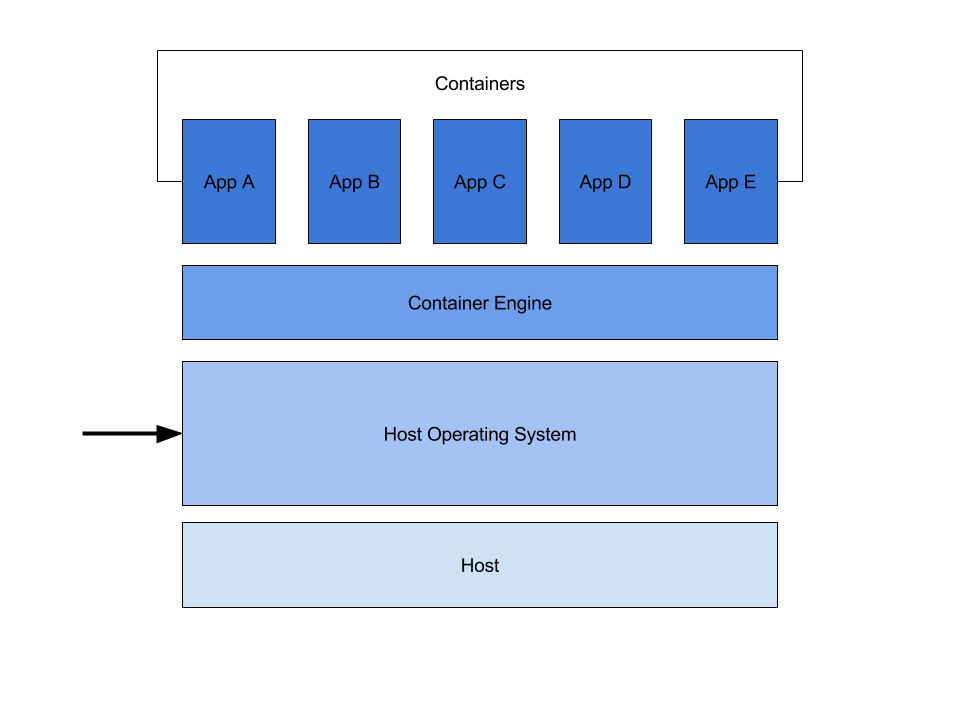
\includegraphics[scale=.4]{architecture}

\section*{Microkernel Architecture}
\subsection*{Minimal Design}

\section*{Container Basics}
\section*{Container Requirements}
\section*{Feasibility}

\bibliography{paper}
\bibliographystyle{IEEEtran}
\end{document}
